%!TEX root = main_ISMB.tex
\section{Supplementary data}
\subsection{RNAinverse}
Using the same dataset of $50$ structures, we generated $100$ samples
per structure with \RNAinverse. They yield for most parameters
a high entropy. Although, the $\texttt{C+G}$ content variation is minimal
through all samples. We show the results when using only \RNAinverse, 
only \texttt{Incarnation}, and both.


\begin{figure}[ht!]
	\centering
	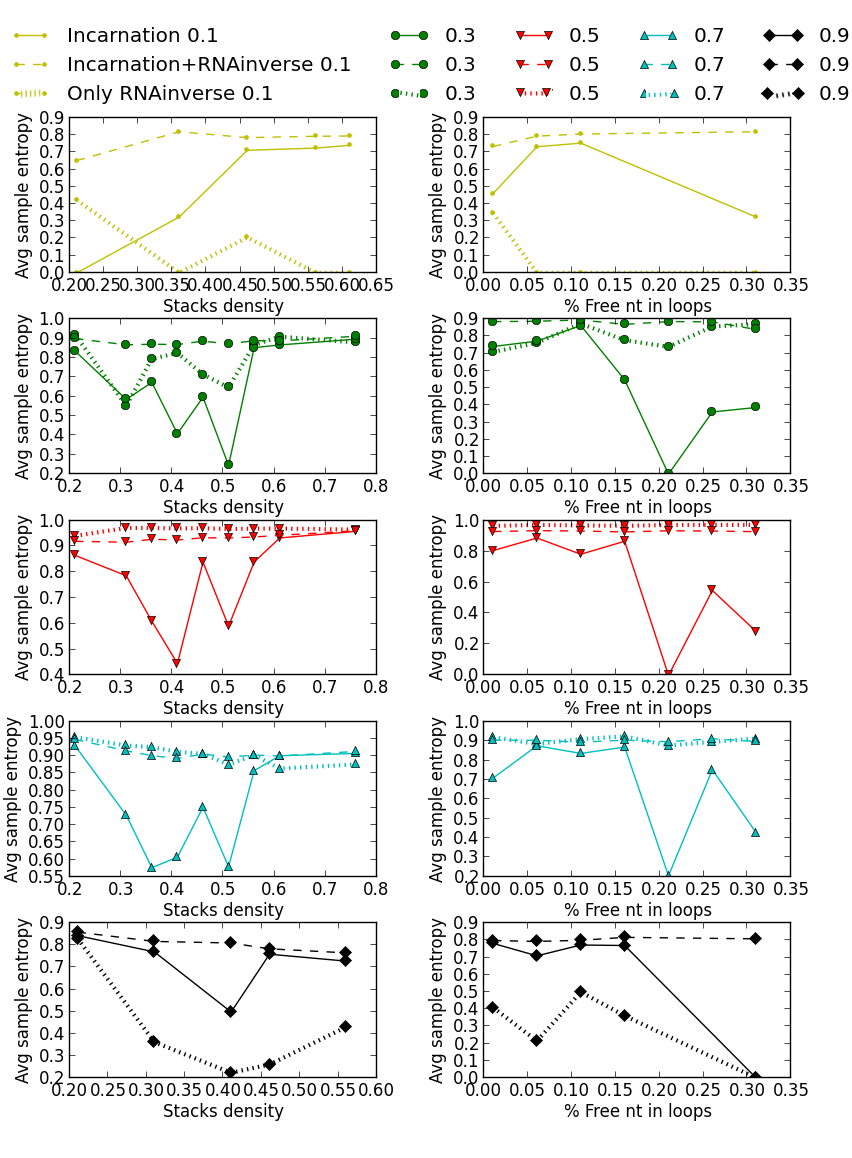
\includegraphics[scale=0.4]{Figures/RNAinverse_data_100.png}
	\caption{Entropy and \texttt{C+G} content. The first
		column is in function of the length, the second of the stacks
		density and the last of the percentage of free nucleotides in loops.
		The blue line represents the results and standard deviation when using 
		only \RNAinverse with 100samples.  The dashed lines are the results
		when using only \texttt{Incarnation} and the dashed line are results
		of \texttt{Incarnation} post-processed by \RNAinverse.
		}
	\label{fig:rnainverse}
\end{figure}